% Short report. Build: pdflatex short_report.tex (twice). Figures are read from ../figures/.
\documentclass[10pt,a4paper]{article}
\usepackage[T1]{fontenc}
\usepackage[utf8]{inputenc}
\usepackage{lmodern}
\usepackage[english]{babel}
\usepackage[a4paper,margin=2.2cm]{geometry}
\usepackage{microtype}
\usepackage{amsmath,amssymb}
\usepackage{graphicx}
\usepackage{booktabs}
\usepackage{array}
\usepackage{caption}
\usepackage{enumitem}
\usepackage{xcolor}
\usepackage[hidelinks]{hyperref}
\graphicspath{{../figures/}}
\captionsetup{font=small,labelfont=bf}
\setlist{itemsep=1pt,topsep=3pt}
\newcommand{\file}[1]{\texttt{\detokenize{#1}}}

\title{\textbf{Can the equations of a physical reservoir\\ predict its computing capacity?}\\[4pt]
\large Preliminary results on simulated substrates}
\author{Niels Faucher}
\date{November 2026 --- work in progress, not peer reviewed}

\begin{document}
\maketitle

\begin{center}
\fcolorbox{black!60}{black!4}{\parbox{0.92\linewidth}{\small\textbf{Status.} This is exploratory
work. All systems are simulated, a single forecasting task is used, and nothing here has been
reviewed by peers. Numbers may change as errors are found. Please read the results as
working hypotheses, not as established facts.}}
\end{center}

\begin{abstract}
\noindent In physical reservoir computing, the dynamics are fixed by the laws of the substrate
and only a linear readout is trained. We ask whether the equations alone, before any training
or driving, tell us whether a substrate will compute well. Our first idea, that a richer or
more complex dynamics computes better, did not survive testing. What did survive is a
\emph{structural} reading of the equations. A filter of four necessary conditions, computed
from the undriven system, separates systems that can forecast a chaotic series from those
that cannot. On 90 systems never seen before, including two new families of substrates, the
median forecast error is 0.28 for admitted systems against 0.56 for rejected ones. Two
quantities computed from the linearised equations add information inside a family: the static
non-linearity at the operating point, and the linear memory capacity, which ranks 40 new
spring networks by forecast error (rank correlation $-0.59$). Five of seven criteria written
before the confirmation run are met; two are not, and are reported as failures.
\end{abstract}

\section{The question}

A reservoir computer passes an input $u(t)$ through a fixed dynamical system,
$\mathbf r(t+1) = f(\mathbf r(t), u(t))$, and trains only a linear readout of the state
\cite{jaeger2001,maass2002,lukosevicius2009}. In \emph{physical} reservoir computing the
system is a piece of matter or a mechanism \cite{tanaka2019}: its equations are given, not
chosen. Selecting a substrate is therefore costly: one builds it, drives it, trains a readout
and measures. We ask whether part of this selection can be done on paper, from the equations.

The task is fixed throughout: forecasting the chaotic Mackey--Glass series \cite{mackey1977}
10 and 20 steps ahead. These horizons were chosen by a rule set in advance: a linear
autoregressive model must fail (NRMSE 0.42 and 0.45) while a non-linear model succeeds (an
echo state network, ESN, reaches 0.10 and 0.085). At one step ahead the linear model already
reaches 0.024, so success there proves nothing. The Lorenz series failed the rule at every
horizon and was not used.

\section{How the idea evolved}

\paragraph{First hypothesis: complexity.} We built an eight-axis \emph{complexity vector}
measured on the reservoir states (permutation entropy, statistical complexity, participation
ratio, neural complexity, relaxation times, conditional Lyapunov exponent, consistency), and
hypothesised that it predicts computing capacity across substrates. Three results ended this
hypothesis.
\begin{enumerate}
  \item \textbf{No transfer.} A map from vector to memory capacity learned on 72 ESNs
        predicted 72 Coulomb-charge reservoirs worse than the mean ($R^2 = -2.59$).
  \item \textbf{A misleading benchmark.} When the readout was trained and tested on the same
        trajectory, the Coulomb system showed a memory capacity of 12.9, higher than the ESN.
        Tested on a run started elsewhere, it dropped to 0.2: the system never forgets its
        initial state, and the readout had learned a trajectory, not a function of the input.
  \item \textbf{Same equations, very different capacities.} Twelve spring networks obey
        identical equations and differ only by their random geometry; their memory capacity
        ranges from 0.5 to 8.3. Adding a cubic term to the springs changes nothing measurable.
        Predicting a held-out geometry failed ($R^2 \le 0.2$).
\end{enumerate}
The algebraic complexity of the equations does not predict performance, and the ``richest''
equations (Coulomb) give the worst reservoir. But the \emph{cause} of that failure can be read
in the equations: an isotropic well makes the system invariant under rotation (a neutral mode),
and mixed-sign charges create many equilibria.

\paragraph{Second hypothesis: structure.} \emph{The structure of a system's equations
(symmetries, dissipation, equilibria, linearised spectrum, non-linearity at the operating
point) predicts its computing capacity, before the system is driven.} We first apply
qualitative necessary conditions (a filter), then ask whether quantitative descriptors explain
the differences that remain. Kept from the first idea: the benchmark corrections and the
consistency axis. Dropped: the claim that one complexity scale works for all substrates.

\section{Methods}

\paragraph{Substrates.} An ESN (50 nodes) serves as a calibration standard, not as a target.
The physical families are simulated: random networks of 25 masses and springs with 6 anchors
\cite{hauser2011}, the random geometry being a hidden parameter; chains of 50 masses in a
single well, a double well, or free; charges in a harmonic well, following the equations of
an $N$-body reservoir by a colleague\footnote{\url{https://github.com/lele394/N-Body-electromagnetic-reservoir-computer}};
and, for the final confirmation only, two families never used before: a single non-linear
node with a delay loop \cite{appeltant2011}, and charges of one sign in an elliptic well.

\paragraph{Benchmark.} The readout (ridge regression) is trained on one simulation and tested
on another one that starts from a different state and receives a different input, with 1\,\%
measurement noise. NRMSE is capped at 1.

\paragraph{Structural filter.} Computed without any time-varying input. The system is relaxed
to rest, and the Jacobian $J$ of one step is obtained by finite differences.
\textbf{Q1}: no neutral mode ($|\mu| < 1 - 10^{-5}$ for all eigenvalues of $J$).
\textbf{Q2}: the system returns to the same state from six random starts.
\textbf{Q3}: the input acts on the state. \textbf{Q4}: the readout sees the state.
A system is \emph{admitted} if all four hold. These are necessary conditions for the echo
state property \cite{jaeger2001}, also known as fading memory \cite{boydchua1985}, convergent
dynamics \cite{pavlov2004} or contraction \cite{lohmiller1998}: a system that forgets its
initial state for every input must do so for zero input. They are local and numerical, not
sufficient.

\paragraph{Quantitative descriptors.} Also computed without driving the system.
(i)~\emph{Linear memory capacity.} Near equilibrium, $\delta\mathbf s(t+1) = J\,\delta\mathbf
s(t) + \mathbf b\,u(t)$ and the read channels are $\mathbf x = C\,\delta\mathbf s$, so
$\mathbf x(t) = \sum_j \mathbf g_j u(t-j)$ with $\mathbf g_j = C J^j \mathbf b$. For i.i.d.\
input,
\begin{equation*}
  \mathrm{MC} = \sum_{k=1}^{80} \mathbf g_k^{\top}\bigl(G + \varepsilon^2 \operatorname{diag} G\bigr)^{-1}\mathbf g_k ,
  \qquad G = \sum_j \mathbf g_j \mathbf g_j^{\top},\quad \varepsilon = 0.01,
\end{equation*}
the classical memory of a noisy linear system \cite{jaeger2002,white2004,ganguli2008,dambre2012},
here applied to the linearisation of a physical substrate. No parameter is fitted.
(ii)~\emph{Static non-linearity}
$\mathrm{nl} = \lVert\Delta\mathbf x(1) - 2\,\Delta\mathbf x(0.5)\rVert / \lVert\Delta\mathbf x(1)\rVert$,
where $\Delta\mathbf x(u)$ is the shift of the equilibrium under a constant input $u$; it is 0
for a linear system. (iii)~\emph{A graded version of Q2}, $d_2$: the spread of final states
divided by the static response amplitude.

\paragraph{Protocol.} Exploration on 64 systems whose performance had already been seen;
there we chose the threshold of a graded rule ($d_2 < 0.01$) and a predictor of the error
(5 nearest neighbours on the descriptors, chosen over ridge regression by leave-one-out).
Both were then frozen. Confirmation on 90 new systems: 40 spring geometries, 12 ESNs at four
input scales, 19 chains, 11 delay nodes, 8 repulsive Coulomb systems. Hypotheses and
numerical criteria were written in the code before the first confirmation system was run.
The error is the mean NRMSE at horizons 10 and 20.

\section{Results}

\paragraph{The filter separates systems that can forecast from those that cannot.} It was
tested three times. On 21 systems used to build it, the median error is 0.12 for admitted
systems against 0.86 for rejected ones; this is exploratory, since two conditions were
reworded after seeing these results. On a first set of 33 unseen systems, 0.16 against 0.35,
with 6 of the 8 best systems admitted; one of the three criteria failed as run, because of a
scale error in Q2, and passed after the fix. On the final set of 90 unseen systems, 0.28
against 0.56, with 17 of the 22 best systems admitted (figure~\ref{fig:filter}). Both new
families behave as predicted: the 8 repulsive Coulomb systems are rejected (seven distinct
final states out of seven) and all fail; the 9 single-state delay nodes are admitted, the
2 bistable ones rejected.

\begin{figure}[!htb]
\centering
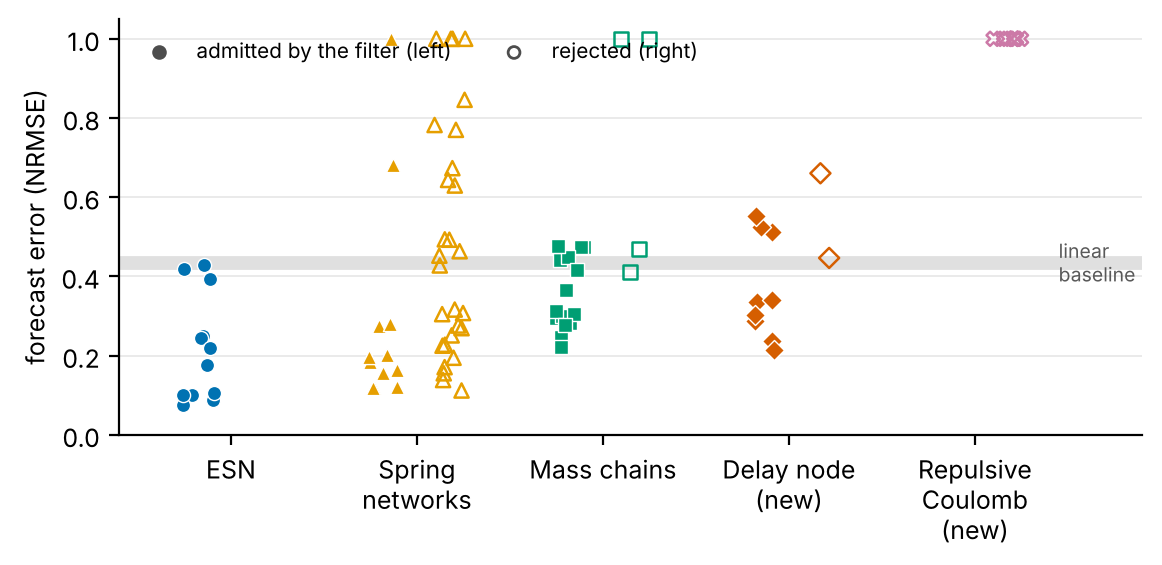
\includegraphics[width=0.9\linewidth]{short_filter.png}
\caption{Forecast error of the 90 confirmation systems, by family. Filled: admitted by the
filter. Open: rejected. Grey band: linear autoregressive baseline.}
\label{fig:filter}
\end{figure}

\paragraph{Memory capacity can be computed from the equations.} For nearly linear systems
($\mathrm{nl} < 0.02$), the measured capacity is within 20\,\% of the prediction in 5 cases
out of 5, with a median deviation of 4\,\% (11\,\% for more non-linear systems). The
deviation always goes the same way: non-linearity lowers the capacity below the linear value
(figure~\ref{fig:mc}). Note that the measurement itself is biased low on short runs (about
$-10\,\%$ at 3\,000 steps), so it was done on 20\,000 steps; this was decided before the test
was run.

\begin{figure}[!htb]
\centering
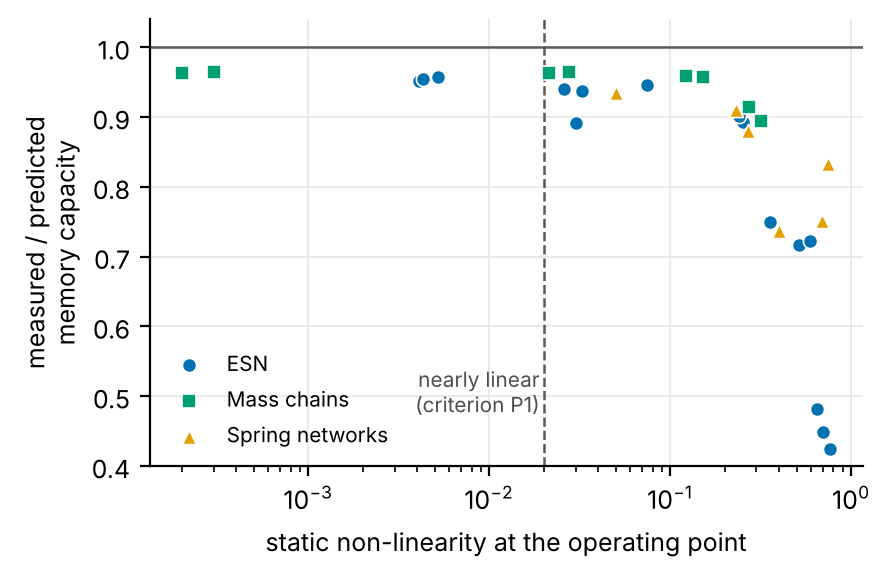
\includegraphics[width=0.55\linewidth]{short_linear_mc.png}
\caption{Ratio of measured to predicted memory capacity for 29 systems, against the static
non-linearity.}
\label{fig:mc}
\end{figure}

\paragraph{An admitted but linear system forecasts no better than a linear model.} The six
admitted systems with $\mathrm{nl} < 0.01$ (three chains at small amplitude, three ESNs at
input scale 0.01) have errors between 0.39 and 0.48, the level of the linear baseline; the
other 42 admitted systems have a median of 0.26 (figure~\ref{fig:quant}a). The same ESN goes
from 0.43 to 0.10 when its input scale rises from 0.01 to 1. For a task that is not linearly
solvable, non-linearity at the operating point acts as a fifth necessary condition.

\paragraph{Inside a family, linear memory ranks the spring networks.} Among the 40 new
geometries, the predicted memory capacity is correlated with the forecast error (rank
correlation $-0.59$; $-0.65$ over all 76 geometries), and the link holds separately among
admitted ($-0.48$) and rejected ($-0.57$) networks (figure~\ref{fig:quant}b). This is the
result that the complexity vector could not deliver. It is a ranking, not a precise
prediction.

\begin{figure}[!htb]
\centering
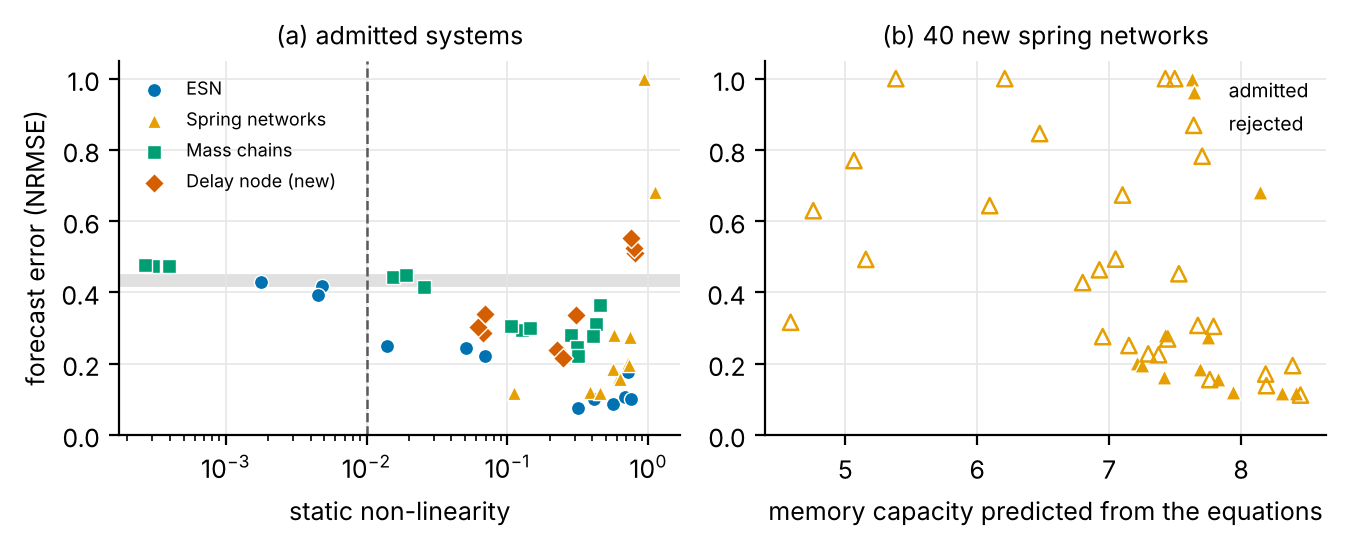
\includegraphics[width=0.95\linewidth]{short_quantitative.png}
\caption{(a) Admitted systems: error against static non-linearity; left of the dashed line,
nearly linear systems. (b) The 40 new spring networks: error against the memory capacity
predicted from the linearised equations.}
\label{fig:quant}
\end{figure}

\paragraph{What failed.} The graded condition $d_2$ does no better than the binary verdict:
several spring networks with two or more final states forecast very well, and neither the
number nor the spread of final states captures why. The frozen predictor beats the family
mean overall but explains only 9\,\% of the variance among springs (threshold: 10\,\%), and
on the delay node, a family it had never seen, it does worse than the plain mean.
Table~\ref{tab:criteria} lists all criteria.

\begin{table}[!htb]
\centering\small
\begin{tabular}{@{}l>{\raggedright\arraybackslash}p{8.3cm}>{\raggedright\arraybackslash}p{3.6cm}l@{}}
\toprule
 & Criterion, written before running & Result & Verdict \\
\midrule
P1 & nearly linear systems: measured MC within 20\,\% of prediction for $\ge 80\,\%$ & 5 of 5 & met \\
P2 & admitted, $\mathrm{nl}<0.01$: $\ge 80\,\%$ have NRMSE $\ge 0.35$, none below 0.25 & 6 of 6, min.\ 0.39 & met \\
P3a & springs: rank correlation (linear MC, error) $\le -0.4$ & $-0.59$ & met \\
P3b & springs, graded rule: median admitted $<$ rejected, $\ge 75\,\%$ of best quarter admitted & 0.20 vs 0.37; 6 of 10 & \textbf{failed} \\
P4a & frozen predictor beats the family mean (squared error) & 0.059 vs 0.089 & met \\
P4b & springs: $R^2$ of the predictor $> 0.1$ & 0.09 & \textbf{failed} \\
P5a & filter: median admitted lower by $\ge 0.10$ & 0.28 vs 0.56 & met \\
P5b & filter: $\ge 75\,\%$ of the best quarter admitted & 17 of 22 & met \\
\bottomrule
\end{tabular}
\caption{Pre-registered criteria. P1 comes from the theory test, P2--P5 from the confirmation
on 90 unseen systems. P3a replaced a hypothesis on $d_2$ after the exploration showed $d_2$
was unrelated to the error among springs ($+0.13$, against $-0.73$ for linear MC); the
change was made and recorded before any confirmation system was run.}
\label{tab:criteria}
\end{table}

\section{Limitations and next steps}

All substrates are simulated; real devices add noise, drift and unmodelled physics. A single
task is used. The 40 spring networks share one operating point. P1 and P2 rest on five and
six systems. The filter is a set of local, numerical necessary conditions; ``structural
analysis'' is a loose name for what is really local stability and basin analysis. A focused
literature search did not find this filter applied across varied physical substrates with a
confirmation on unseen systems, but the search was not exhaustive; the closest approaches
characterise substrates from data \cite{dale2019}. Multistability, rejected here, is used
elsewhere as a resource for storing several behaviours \cite{terajima2025}: the filter is
meant for input-driven forecasting only.

Next steps: (1) test Q2 \emph{under a constant input}, since the admitted systems that fail
completely are those with the strongest static non-linearity, which suggests the input pushes
them into another state; (2) understand why some multi-state systems forecast well;
(3) extend the memory-based ranking to other families with hidden parameters; (4) autonomous
forecasting of Lorenz, not yet attempted.

\paragraph{Code.} Every number and figure above comes from the code in this repository
(\file{src/}, steps 1--17); figures are redrawn from \file{data/} by
\file{report/make_figures.py}. Code and text were developed with the help of an AI assistant;
all results come from executed code.

\small
\begin{thebibliography}{99}\setlength{\itemsep}{0pt}
\bibitem{appeltant2011} L.~Appeltant et al., Information processing using a single dynamical node as complex system, \emph{Nat.\ Commun.}\ 2, 468 (2011).
\bibitem{boydchua1985} S.~Boyd, L.~O.~Chua, Fading memory and the problem of approximating nonlinear operators with Volterra series, \emph{IEEE Trans.\ Circuits Syst.}\ 32, 1150 (1985).
\bibitem{dale2019} M.~Dale, J.~F.~Miller, S.~Stepney, M.~A.~Trefzer, A substrate-independent framework to characterize reservoir computers, \emph{Proc.\ R.\ Soc.\ A} 475, 20180723 (2019).
\bibitem{dambre2012} J.~Dambre, D.~Verstraeten, B.~Schrauwen, S.~Massar, Information processing capacity of dynamical systems, \emph{Sci.\ Rep.}\ 2, 514 (2012).
\bibitem{ganguli2008} S.~Ganguli, D.~Huh, H.~Sompolinsky, Memory traces in dynamical systems, \emph{PNAS} 105, 18970 (2008).
\bibitem{hauser2011} H.~Hauser, A.~J.~Ijspeert, R.~M.~F\"uchslin, R.~Pfeifer, W.~Maass, Towards a theoretical foundation for morphological computation with compliant bodies, \emph{Biol.\ Cybern.}\ 105, 355 (2011).
\bibitem{jaeger2001} H.~Jaeger, The ``echo state'' approach to analysing and training recurrent neural networks, GMD Report 148 (2001).
\bibitem{jaeger2002} H.~Jaeger, Short term memory in echo state networks, GMD Report 152 (2002).
\bibitem{lohmiller1998} W.~Lohmiller, J.-J.~E.~Slotine, On contraction analysis for non-linear systems, \emph{Automatica} 34, 683 (1998).
\bibitem{lukosevicius2009} M.~Luko\v{s}evi\v{c}ius, H.~Jaeger, Reservoir computing approaches to recurrent neural network training, \emph{Comput.\ Sci.\ Rev.}\ 3, 127 (2009).
\bibitem{maass2002} W.~Maass, T.~Natschl\"ager, H.~Markram, Real-time computing without stable states, \emph{Neural Comput.}\ 14, 2531 (2002).
\bibitem{mackey1977} M.~C.~Mackey, L.~Glass, Oscillation and chaos in physiological control systems, \emph{Science} 197, 287 (1977).
\bibitem{pavlov2004} A.~Pavlov, A.~Pogromsky, N.~van de Wouw, H.~Nijmeijer, Convergent dynamics, a tribute to B.~P.~Demidovich, \emph{Syst.\ Control Lett.}\ 52, 257 (2004).
\bibitem{tanaka2019} G.~Tanaka et al., Recent advances in physical reservoir computing: a review, \emph{Neural Netw.}\ 115, 100 (2019).
\bibitem{terajima2025} R.~Terajima, K.~Inoue, K.~Nakajima, Y.~Kuniyoshi, Multifunctional physical reservoir computing in soft tensegrity robots, arXiv:2507.21496 (2025).
\bibitem{white2004} O.~L.~White, D.~D.~Lee, H.~Sompolinsky, Short-term memory in orthogonal neural networks, \emph{Phys.\ Rev.\ Lett.}\ 92, 148102 (2004).
\end{thebibliography}
\end{document}
